\documentclass[letterpaper,10pt]{article}

\usepackage[utf8]{inputenc}
\usepackage[spanish]{babel}
\usepackage{fontenc}
\usepackage[dvipdfmx]{graphicx}
\usepackage{bmpsize,wrapfig,xcolor}
\usepackage{fullpage}
\usepackage[hidelinks]{hyperref}
\usepackage{subcaption}

% Para evitar que se indente solo a cada rato
\setlength\parindent{0pt}

\begin{document}
	\begin{titlepage}

		\begin{wrapfigure}{R}{0.3\textwidth}
			
\includegraphics[width=0.3\textwidth]{logoFCFM.png}
		\end{wrapfigure}

		\noindent \phantom - % "Hax" para que quede alineada la imagen con el texto

		Universidad de Chile

		Facultad de Ciencias Físicas y Matemáticas

		Depto. de Ciencias de la Computación

		CC5208 - Visualización de Información

		\vfill

		\begin{center}
			\begin{Huge}
				{\textbf{Tarea 3}}
			\end{Huge}

			\begin{large}
				Layout del proyecto
			\end{large}

		\end{center}
--
		\vfill

		\begin{flushright}
			\begin{tabular}{lll}
				Integrantes	&:	& Américo Ferrada\\
						&:	& Gabriel Sanhueza\\
				Profesor	&:	& Javier Bustos\\
				Ayudante	&:	& Diego Madariaga\\
				Repositorio GitHub &:	& \url{https://github.com/gsanhueza/Tarea3Visualizacion}\\
			\end{tabular}
		\end{flushright}

	\end{titlepage}

	% % % % % % % % % % % % % % % % % % % % % % % % % % % % % % % % % % % % % % % % % % % % % % % % % % % % % % % % % % % % % % % % % % % % % % % % % % % % % % % % % % % % % % % % % %
	\newpage
	% % % % % % % % % % % % % % % % % % % % % % % % % % % % % % % % % % % % % % % % % % % % % % % % % % % % % % % % % % % % % % % % % % % % % % % % % % % % % % % % % % % % % % % % % %

	\tableofcontents

	% % % % % % % % % % % % % % % % % % % % % % % % % % % % % % % % % % % % % % % % % % % % % % % % % % % % % % % % % % % % % % % % % % % % % % % % % % % % % % % % % % % % % % % % % %
	\newpage
	% % % % % % % % % % % % % % % % % % % % % % % % % % % % % % % % % % % % % % % % % % % % % % % % % % % % % % % % % % % % % % % % % % % % % % % % % % % % % % % % % % % % % % % % % %

	\section{Análisis}

	\subsection{Tipo de datos}

	Existen 10 columnas de datos en total:

	\begin{itemize}
		\item Nombre: Aleatorio
		\item Id: Ordinal
		\item Tipo: Categórico
		\item Clase: Categórico
		\item Masa: Ordinal

		\item Caído/Encontrado: Categórico
		\item Año: Ordinal
		\item Latitud: Ordinal
		\item Longitud: Ordinal
		\item Geolocalización: Ordinal (Tupla)
	\end{itemize}

	\subsection{Relaciones entre datos}

	Nuestros datos se relacionan de la siguiente manera:

	\begin{itemize}
		\item Tamaño y tipo del meteorito: Cada tipo de meteorito depende de su tamaño.
		\item Cantidad de meteoritos y año encontrado: Entre más reciente, mayor es la cantidad de meteoritos encontrados.
		\item Tamaño de los meteoritos y geolocalización: Se encuentra mayor cantidad de meteoritos pequeños en los polos.
		\item Nombre propio y tamaño del meteorito: Los meteoritos de tamaño no-despreciable tienen nombre propio (Ej.: Alessandria) v/s los más pequeños (Ej.: Yamato 983824)
	\end{itemize}

	% % % % % % % % % % % % % % % % % % % % % % % % % % % % % % % % % % % % % % % % % % % % % % % % % % % % % % % % % % % % % % % % % % % % % % % % % % % % % % % % % % % % % % % % % %
	\newpage
	% % % % % % % % % % % % % % % % % % % % % % % % % % % % % % % % % % % % % % % % % % % % % % % % % % % % % % % % % % % % % % % % % % % % % % % % % % % % % % % % % % % % % % % % % %

	\section{Planteamiento de preguntas}

	Preguntas que esperamos responder con nuestra visualización:


	\begin{enumerate}
		\item ¿Dónde se encuentran más meteoritos en función del peso?
		\item ¿Cuál es el tipo de meteoritos más frecuente? % Contador vs Tipos
		\item Respecto al peso, ¿cuáles son los tipos de meteoritos encontrados? % Peso vs Tipo

		\item ¿Cuál es el peso de meteorito más frecuente?
		\item ¿Cuáles son los 10 meteoritos más pesados encontrados?
		\item ¿Cuáles son los 10 meteoritos más livianos encontrados?

		\item ¿En qué año se encontraron más meteoritos?
		\item ¿En qué pais se han encontrado más meteoritos?
		\item ¿Cuál es el tipo de meteorito más frecuente en función de su geolocalización?
	\end{enumerate}

	\section{Mapeo datos a gráficos}

	Como relacionar los datos para responder las preguntas anteriores:

	\begin{enumerate}
		\item Basta mapear los datos (geolocalización) en varios mapas mundiales separados por segmentos de peso, cuadricular cada mapa y mostrar con distintos colores según densidad
		de meteoritos por cada cuadro.
		\item En un gráfico de barra, por cada tipo contar sus apariciones.
		\item En un gráfico de barra, tomando solo un segmento de los datos en función del peso.

		\item En un scatterplot, ordenar los meteoritos en función del peso y contar sus ocurrencias.
		\item Se usa gráfico anterior.
		\item Se usa gráfico anterior.

		\item En un scatterplot, contar apariciones de meteoritos en función del año.
		\item Dado un mapa mundial, utilizar un gradiente de color en función del número de meteoritos caídos por país.
		\item Dado un mapa mundial, utilizar un gradiente de color en función del número de meteoritos caídos por tipo.
	\end{enumerate}

	% % % % % % % % % % % % % % % % % % % % % % % % % % % % % % % % % % % % % % % % % % % % % % % % % % % % % % % % % % % % % % % % % % % % % % % % % % % % % % % % % % % % % % % % % %
	\newpage
	% % % % % % % % % % % % % % % % % % % % % % % % % % % % % % % % % % % % % % % % % % % % % % % % % % % % % % % % % % % % % % % % % % % % % % % % % % % % % % % % % % % % % % % % % %

	\section{Diseño}
	% TODO Diseño

	\subsection{Mapa Mundial}

	Se eligió un mapa mundial, dado que las preguntas de ubicación geográfica se responden mucho más fácilmente así, en lugar de usar un gráfico de barras o de líneas.

	En particular, se decidió usar un mapa mundial mudo para poder aprovechar el procesamiento \textit{pre-attentive} de las personas, distinguiendo por color los datos y sacando del
	foco al mar, donde no hay información para mostrar.

	Para los datos de geolocalización, se eligió una paleta de colores entre los colores rojo y azul, puesto que son intuitivos para los gradientes (azul es menos, rojo es más).

	Por último, usando la Ley de la Experiencia (Gestalt), un mapa mundial está presente en las mentes de las personas, por lo que es posible identificar lugares con más/menos meteoritos
	sin tener que detenerse a pensar dónde cayeron en la realidad.

	\subsubsection{Distribución de meteoritos en el mundo}

	Para este caso, el mapa mundial será dividido en cuadrículas, de forma de poder mostrar genéricamente en que sectores hay una mayor cantidad de meteoritos.

	\subsubsection{Conteo de meteoritos por país}

	Para este caso, el mapa mundial será dividido por países, de forma de poder mostrar los meteoritos caídos por cada nación.

	\begin{tabular}{cc}
		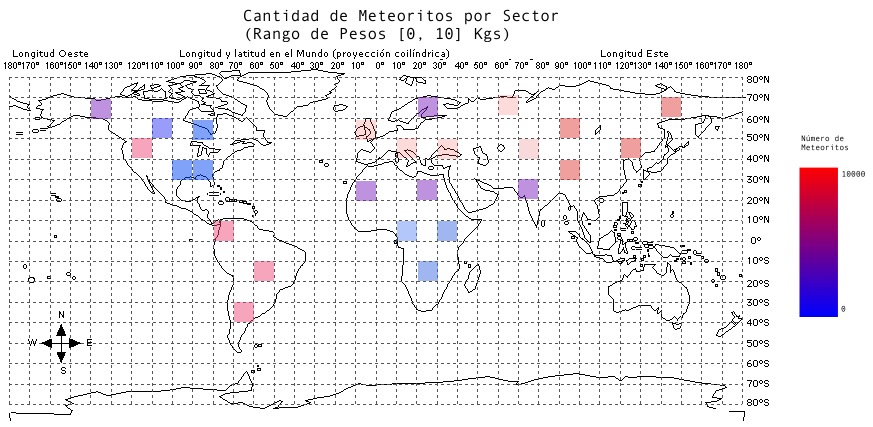
\includegraphics[width=0.5\textwidth]{mapamundiQuad.png} & 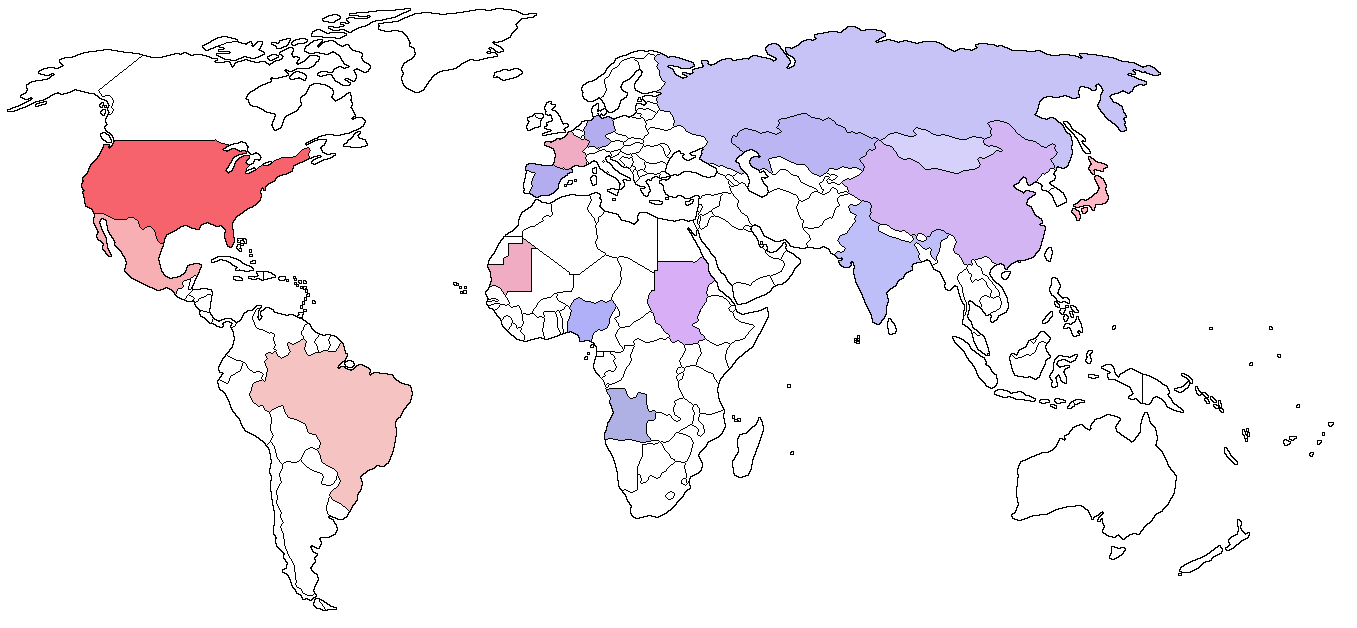
\includegraphics[width=0.5\textwidth]{mapamundiPol.png}\\
		(a) Cuadriculado & (b) Por país\\
	\end{tabular}

	% % % % % % % % % % % % % % % % % % % % % % % % % % % % % % % % % % % % % % % % % % % % % % % % % % % % % % % % % % % % % % % % % % % % % % % % % % % % % % % % % % % % % % % % % %
	\newpage
	% % % % % % % % % % % % % % % % % % % % % % % % % % % % % % % % % % % % % % % % % % % % % % % % % % % % % % % % % % % % % % % % % % % % % % % % % % % % % % % % % % % % % % % % % %

	\subsection{Gráfico de barras / Scatterplot}

	Se eligió usar un gráfico de barras y scatterplot para varias preguntas distintas, por que es la forma más óptima de comparar cantidades, en particular porque las comparación entre alturas
	son intuitivamente reconocidas por la percepción humana, y las variables mostradas en scatterplot permiten encontrar clusters fácilmente (Ley de Proximidad - Gestalt).

	\subsubsection{Tipo}
	Para el tipo, como son las categorias, éstas se puede ordenar lexicográficamente para después mostrar el tipo de meteorito con mayor numero de ocurrencias.

	\begin{center}
		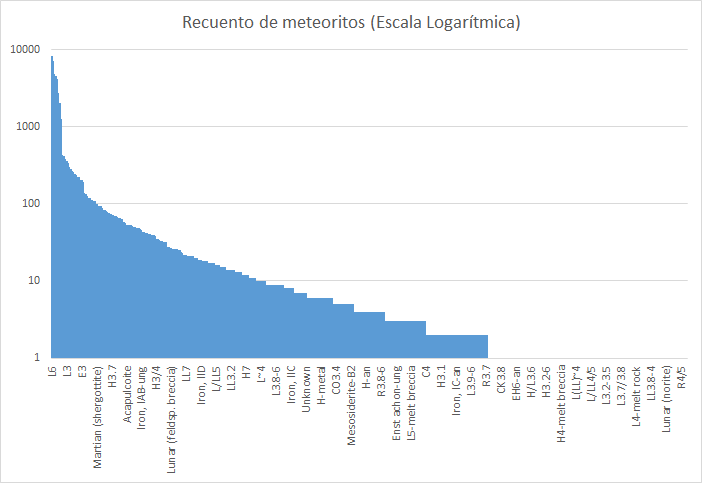
\includegraphics[width=0.4\textwidth]{recurrentes2.png}
	\end{center}

	\subsubsection{Año}
	Para el año, éste se ordena en el eje X, y se compara temporalmente con el numero de meteoritos encontrados.

	\begin{center}
		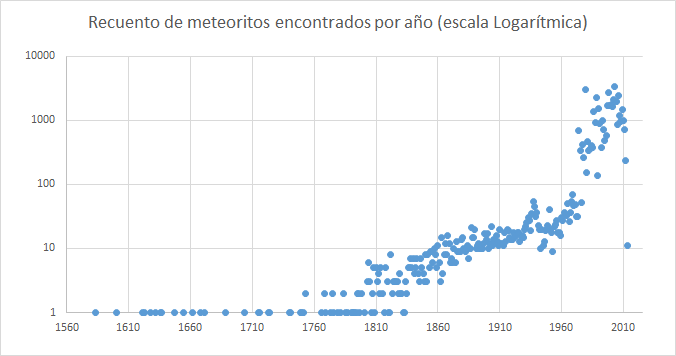
\includegraphics[width=0.4\textwidth]{year2.png}
	\end{center}

	\subsubsection{Peso}
	Para el peso, éste se ordena en el eje X para comparar la cantidad de veces que fueron contados los rangos de pesos elegidos.

	\begin{center}
		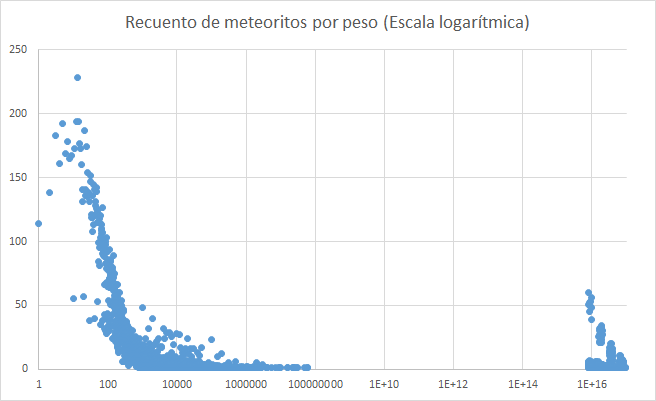
\includegraphics[width=0.4\textwidth]{masa2.png}
	\end{center}

	% 	Paleta de colores: http://paletton.com/#uid=50K0D0kS-C8tqT2FFTwQPquQols

\end{document}
